% Yantra — arXiv preprint source.
% Self-contained: article class + standard packages only, embedded
% bibliography (no BibTeX run needed), figures in ./figs/.
% Compile: pdflatex main.tex (twice for references) or any LaTeX engine.
\documentclass[11pt]{article}

\usepackage[T1]{fontenc}
\usepackage{lmodern}
\usepackage[margin=1in]{geometry}
\usepackage{amsmath,amssymb}
\usepackage{graphicx}
\usepackage{booktabs}
\usepackage{listings}
\usepackage{xcolor}
\usepackage[hidelinks]{hyperref}

\lstset{
  basicstyle=\small\ttfamily,
  breaklines=true,
  breakatwhitespace=true,
  columns=fullflexible,
  keepspaces=true,
  frame=single,
  rulecolor=\color{black!30},
  backgroundcolor=\color{black!3},
}
\newcommand{\code}[1]{\texttt{#1}}
\newcommand{\GH}{\url{https://github.com/eulogik/yantra}}
\newcommand{\HF}{\url{https://huggingface.co/eulogik/yantra-1b-agent}}

\title{Yantra: A Reproducible Recipe for Sub-1B Agentic Tool Calling\\with Decoupled Routing}
\author{Gautam Kishore\\
  \texttt{gautam@eulogik.com}\\
  \and
  %% TODO: add co-authors here if any
}
\date{September 14, 2026}

\begin{document}
\maketitle

\begin{abstract}
Small language models struggle with agentic tool calling when a single
forward pass must jointly select a tool, fill its arguments, and stop
cleanly---especially under generic serving stacks that differ from a
model's native runtime. We present Yantra, a fully reproducible recipe
that turns a 1\,B-parameter model into a reliable single-call tool user
on a free Colab T4 with zero paid API calls. The core idea,
\emph{Decoupled Tool Selection / Argument Generation} (DTSA), moves
tool choice into a cheap, testable runtime router
(IDF $+$ char-3-gram $+$ embedding blend, 247/300 routing accuracy)
and trains the language model to emit \emph{only} the arguments inside
a strict bind/args/action-end contract enforced by fixed
stop sequences. On a deterministic 300-case ToolACE slice, Yantra
reaches a Primary Aggregated Score (PAS) of \textbf{0.6775} against
\textbf{0.1922} for an identically served reference agentic model
($3.52\times$), with 100\% parseable output and 65\% exact-argument
accuracy. We release the Q4\_K\_M weights (688\,MB, MIT), the training
and evaluation pipeline, and---unusually---a documented negative
result: small-data contrastive training (66 pairs) collapses argument
quality, while supervised replay on the same fixes recovers safely.
Scope is deliberately narrow (single-call, English, $n=300$); we state
every threat to validity inline so the work can be built on without
surprises.
\end{abstract}

\noindent\textbf{Artifacts:} code \GH{} \\
weights \HF{} \\
License: MIT (code and Yantra weights; base model Apache-2.0).

%=====================================================================
\section{Introduction}
\label{sec:intro}

Function calling---having a language model invoke external tools and
APIs---is the foundation of language agents, enterprise workflows, and
on-device assistants~\cite{bfcl,gorilla,toolllm}. Frontier models do it
well, but the devices where agents would be most useful (phones,
laptops, edge hardware) cannot run them. Small language models (SLMs)
are the natural answer~\cite{minicpm}, yet a 1\,B model asked to read a
tool list, pick the right tool, fill every argument correctly, and stop
generating---all in one shot---fails in mundane, system-breaking ways:
it echoes the tool schema back, mangles argument tags, invents
follow-up turns, or never emits a stop token. The failure is sharpest
under \emph{generic serving}: a model trained for one runtime (e.g.\
SGLang with a native parser) degrades badly when served through another
(e.g.\ llama.cpp), which is exactly the situation an open,
reproducible project faces.

This paper asks a practical question: \emph{with one free Colab T4 GPU,
zero paid API calls, and a 1\,B base model, how far can careful
systems engineering plus lightweight fine-tuning move single-call tool
accuracy?} Our answer is Yantra, a recipe rather than just a
checkpoint:

\begin{enumerate}
  \item \textbf{DTSA (Decoupled Tool Selection / Argument Generation).}
    Tool choice is removed from the language model entirely. A runtime
    router binds \code{<bind tool="..."/>}; the model generates only
    the \code{<args>} block closed by \code{<action\_end/>}.
    Routing accuracy
    becomes an independent, GPU-free engineering target.
  \item \textbf{Router V2 + embedding blend.} An IDF-weighted lexical
    scorer with char-3-gram name matching (244/300), blended
    50/50 with MiniLM cosine similarity (247/300), with per-query
    normalization. No retraining required to upgrade routing.
  \item \textbf{A strict generation contract.} Fixed stop sequences and
    a last-bind-with-args parser (with a tagless fallback) take stopped
    cleanly from 0.12 to 1.00.
  \item \textbf{A metric and protocol that fit the claim.} PAS, the
    mean of eight sub-metrics, on a deterministic 300-case ToolACE
    slice (seed 42), with temperature 0 and a fully scripted harness.
  \item \textbf{Full reproducibility and honest negatives.} Every
    stage reruns on a free T4; weights, code, and notebooks are public.
    A collapsed DPO round (66 pairs) is reported with numbers, not
    buried.
\end{enumerate}

On ToolACE-300, Yantra scores PAS \textbf{0.6775} versus
\textbf{0.1922} for the reference agentic 1\,B model served
identically ($3.52\times$), is parseable on 100\% of cases, and gets
arguments exactly right 65\% of the time. We do \emph{not} claim
state of the art against 7\,B$+$ models, multi-turn planning, or
external benchmarks we did not run (notably BFCL); Section~\ref{sec:limits}
lists every limitation we know. The intended contribution is a
solid, reusable systems recipe at the 1\,B scale---and evidence about
which cheap interventions actually move the needle.

%=====================================================================
\section{Related Work}
\label{sec:related}

\paragraph{Tool-use language models.}
Toolformer~\cite{toolformer} showed LMs can teach themselves API use
via self-supervised data; ReAct~\cite{react} interleaves reasoning
traces with actions for multi-step tasks. Gorilla~\cite{gorilla}
fine-tunes a 7\,B model for API calls and pairs it with a document
retriever for test-time adaptation, evaluating on APIBench.
ToolLLM~\cite{toolllm} scales this to 16k$+$ real APIs with
depth-first-search annotation (DFSDT) and a neural API retriever.
Yantra differs in two ways: routing is \emph{hard-decoupled} from
generation through an explicit bind contract (the LM never sees tool
selection as its job), and the whole recipe runs free on a single T4
with no teacher-API budget. We also deliberately stay single-shot:
unlike ReAct-style traces, there is no reasoning scratchpad, which
keeps 1\,B outputs short and parseable at the cost of no planning.

\paragraph{Data and benchmarks.}
Our training and evaluation data derive from ToolACE~\cite{toolace},
an agentic pipeline (self-evolution synthesis, multi-agent dialog
generation, dual-layer verification) producing 26,507 APIs and
verified dialogs; its 8\,B model rivals GPT-4-class function calling.
For measurement, the Berkeley Function-Calling Leaderboard
(BFCL)~\cite{bfcl} is the de-facto standard (AST-based grading,
multilingual and multi-turn tracks), and APIBank~\cite{apibank} covers
full plan-retrieve-execute workflows. We evaluate on a ToolACE slice
rather than BFCL because our harness, format, and single-call scope
were built around ToolACE from day one; a BFCL port is explicit future
work (Section~\ref{sec:limits}), and we make no cross-benchmark
claims.

\paragraph{Small models and efficient tuning.}
Our base, MiniCPM5-1\,B~\cite{minicpm,minicpm5}, is a 1.08\,B-parameter
Llama-architecture causal LM (24 layers, grouped-query attention,
131\,K native context, Apache-2.0) from the MiniCPM family, whose
training methodology (wind-tunnel scaling, WSD scheduling) targets
strong SLMs~\cite{minicpm}. Notably, its own post-training uses RL
plus on-policy distillation, and its card documents native XML-style
tool calling served via SGLang---a fact central to our baseline
discussion in Section~\ref{sec:baseline}. We fine-tune with
QLoRA~\cite{qlora} ($r{=}64$, $\alpha{=}128$) and use Direct Preference
Optimization~\cite{dpo} in one stage; Section~\ref{sec:negatives}
contributes a cautionary datapoint on DPO with tiny contrastive sets.

%=====================================================================
\section{Method}
\label{sec:method}

Figure~\ref{fig:arch} overviews the system: a decoupled inference path
(top) and the training pipeline that produces the weights (bottom).

\begin{figure}[t]
  \centering
  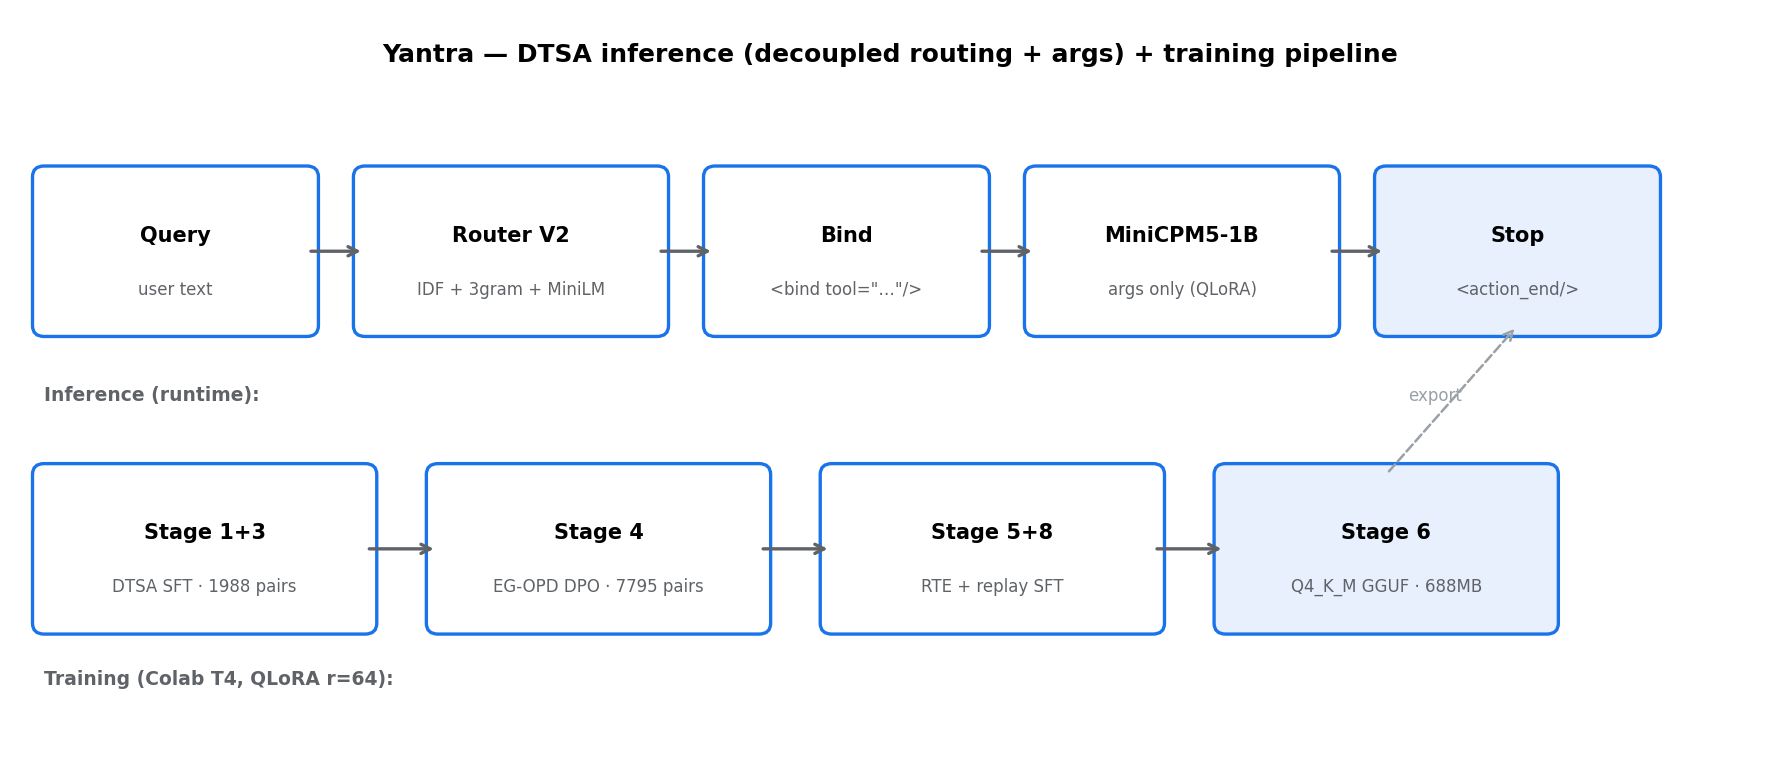
\includegraphics[width=\linewidth]{figs/architecture.png}
  \caption{DTSA inference (top): the router binds the tool, the 1\,B
    model emits arguments only, fixed stops terminate generation.
    Training (bottom): SFT, preference optimization, error-recovery
    SFT, replay, and GGUF export on a Colab T4.}
  \label{fig:arch}
\end{figure}

%---------------------------------------------------------------------
\subsection{DTSA: decoupled tool selection / argument generation}
\label{sec:dtsa}

Given a user query $q$ and a candidate tool list
$T = \{t_1, \dots, t_k\}$ (JSON schemas with names and descriptions),
a conventional agent prompts the LM with $(q, T)$ and asks it to
produce the complete call. DTSA splits this into two contracts.
First, a deterministic router picks
\begin{equation}
  t^* = \operatorname{route}(q, T),
\end{equation}
and the runtime binds it. The LM is then prompted with
\begin{lstlisting}
<user>{q}</user>
<tools>{T as JSON}</tools>
<calls><bind tool="{t*}"/>
\end{lstlisting}
and must complete \emph{only} the argument block:
\begin{lstlisting}
<args><param name="k1">v1</param>...</args><action_end/>
\end{lstlisting}
The split has three consequences. (1)~The LM's task collapses from
open-ended tool reasoning to schema-constrained slot filling, which is
within a 1\,B model's reach. (2)~Routing accuracy is measurable
\emph{without any LLM call} (gold tools are known), so router
improvements are cheap, exact, and decoupled from training.
(3)~Upgrading the router never invalidates the weights.

\subsection{Router V2 with embedding blend}
\label{sec:router}

Let $\mathrm{tok}(s)$ be lowercase alphanumeric tokens and
$\mathrm{tri}(s)$ character 3-grams. Over a tool registry with
documents $d_i = \mathrm{tok}(\mathrm{name}_i + \mathrm{description}_i)$,
inverse document frequencies are
$\mathrm{idf}(w) = \log(N / (1 + \mathrm{df}(w)))$.
For query $q$ with $Q_t = \mathrm{tok}(q)$, $Q_g = \mathrm{tri}(q)$,
tool $t$ scores
\begin{equation}
  s_{\mathrm{lex}}(q,t) =
  \frac{\sum_{w \in Q_t \cap d_t}\mathrm{idf}(w)}
       {\sqrt{\sum_{w \in d_t}\mathrm{idf}(w)} + \epsilon}
  + 2.0\,
  \frac{|Q_g \cap \mathrm{tri}(\mathrm{name}_t)|}
       {\sqrt{|Q_g|\cdot|\mathrm{tri}(\mathrm{name}_t)|} + 1}.
  \label{eq:lex}
\end{equation}
IDF statistics are fit once over the full registry
(\code{fit\_corpus}) and reused for per-query subsets, mirroring the
benchmark construction. Optionally, cosine similarities
$s_{\mathrm{emb}}$ from \code{all-MiniLM-L6-v2} (tool text
``name --- description'') are min-max normalized per query alongside
$s_{\mathrm{lex}}$ and blended as
$(1-\beta)\,s_{\mathrm{lex}} + \beta\,s_{\mathrm{emb}}$ with
$\beta = 0.5$ chosen by sweep. Lexical-only routing needs zero extra
downloads; the blend costs one 80\,MB embedding model at runtime.

\subsection{Training pipeline}
\label{sec:training}

Base model MiniCPM5-1\,B is fine-tuned with QLoRA
($r{=}64$, $\alpha{=}128$, dropout $0.05$) through the stages in
Table~\ref{tab:stages}. Prompts carry the router's bind; completions
are args-only, exactly matching inference. A second DPO round on 66
mined argument failures is \emph{excluded} from the released weights:
it collapsed (Section~\ref{sec:negatives}); a supervised replay step
on the same fixes plus 200 replay rows was used instead. The final
adapter is merged and exported to Q4\_K\_M GGUF (688\,MB). Total
compute is roughly 3 hours on a free Colab T4; no paid teacher or
data-generation APIs are used at any stage.

\begin{table}[t]
  \centering
  \caption{Training stages (Colab T4, QLoRA). Stage numbering follows
    the pipeline notebook; the collapsed DPO round is omitted from the
    released weights and analyzed in Section~\ref{sec:negatives}.}
  \label{tab:stages}
  \begin{tabular}{lllccc}
    \toprule
    Stage & Method & Data & Epochs & LR & Time \\
    \midrule
    1 & Data builder & ToolACE extract & --- & --- & 5\,min \\
    3 & DTSA SFT & 1,988 pairs & 2 & $10^{-4}$ & 30\,min \\
    4 & EG-OPD DPO & 7,795 pairs & 1 & $5{\times}10^{-5}$ & 2\,h \\
    5 & RTE SFT & error corrections & 1 & $10^{-4}$ & 15\,min \\
    8 & SFT replay & 66 fixes $+$ 200 replay & 1 & $10^{-5}$ & 10\,min \\
    6 & Export & Q4\_K\_M GGUF & --- & --- & 10\,min \\
    \bottomrule
  \end{tabular}
\end{table}

\subsection{Inference contract}
\label{sec:inference}

Decoding uses temperature 0, $n_{\mathrm{ctx}}{=}4096$ (of 131\,K
native), \code{max\_tokens} 768, and six fixed stop strings
(newline-bind, tool-result, user, end-calls, tool-error, reflect;
Appendix~\ref{app:prompt}).
The parser takes the \emph{last} bind with an argument block (later
binds supersede earlier ones) and falls back to tagless
\code{name="k">v} lines, because the base tokenizer
treats \code{<param>} as special tokens and may strip them. Generation
is graded on prompt-bind $+$ completion jointly, since the completion
is args-only by construction.

%=====================================================================
\section{Evaluation Protocol}
\label{sec:eval}

\subsection{ToolACE-300}
\label{sec:dataset}

We extract single-call ToolACE dialogs (7,822 parseable of 11,300;
4,382 single-call) and sample a deterministic 300-case set (seed 42).
Each case holds a query, a candidate tool list, and one gold call.
Cases are single-call and English only. The set, builder script, and
seed are released so the exact slice rebuilds bit-for-bit given the
upstream dataset snapshot.

\subsection{PAS: Primary Aggregated Score}
\label{sec:pas}

Let a prediction be graded on six measured components---parseable,
valid tool name, expected (gold) tool name, exact argument match
(keys \emph{and} values), argument-key overlap, stopped
cleanly---each in $[0,1]$, plus recovery and multiturn, currently
unsupported and fixed at 0 (Appendix~\ref{app:pas}). PAS is their
unweighted mean:
\begin{equation}
  \mathrm{PAS} = \tfrac{1}{8}\,
  (m_{\mathrm{parse}} + m_{\mathrm{valid}} + m_{\mathrm{expect}}
  + m_{\mathrm{exact}} + m_{\mathrm{overlap}} + m_{\mathrm{stop}}
  + 0 + 0).
  \label{eq:pas}
\end{equation}
Equal weighting is a deliberate choice: it rewards usable systems
(parseable, correct tool, correct args, clean stop) without letting
any single axis dominate, and the two zero components penalize the
headline honestly for missing capabilities instead of hiding them.

\subsection{Baseline and the serving caveat}
\label{sec:baseline}

Our reference is the public agentic 1\,B baseline
(MiniCPM5 agentic-tooluse GGUF, Q4\_K\_M)\footnote{Repository:
\url{https://huggingface.co/ewinregirgojr/MiniCPM5-1B-Agentic-Tooluse-GGUF}.},
served through llama.cpp with the identical harness, prompts, and
stops as Yantra. It scores PAS \textbf{0.1922}. Its characteristic
failure under this serving is emitting schema echoes or mangled calls
(e.g.\ bare \code{name="...">} fragments) rather than the trained
format. This is \emph{expected}: the baseline targets SGLang's native
\code{minicpm5} stack (its model card documents a dedicated
tool-call parser), which was unavailable in our environment. Its
card-claimed numbers therefore cannot be reproduced through llama.cpp,
and we do not try. Our claim is strictly \textbf{system-vs-system
under identical serving}: Yantra beats the reference $3.52\times$ when
both are served the same way. This is the relevant comparison for
practitioners who must deploy through generic inference stacks.

Because the reference outputs are parser-sensitive under generic
serving (tolerant vs.\ strict parsing moves its sub-metrics while its
headline stays poor), we report \emph{only} its headline PAS from the
controlled baseline run and omit its sub-metric row. This avoids
mixing harnesses in one table---a comparison the reader could not
verify.

\subsection{Reproducibility}
\label{sec:repro}

All runs use temperature 0 and fixed seeds; the pipeline notebook is
resumable (completed stages auto-skip after preemptions). Router
benchmarks run \emph{before} any LLM eval (gold labels known), and the
final eval promotes results only if PAS improves (guarded promote).
Per-case predictions for the official run are retained with the run
artifacts; the repository ships the harness, seeds, and the exact
notebooks.

%=====================================================================
\section{Results}
\label{sec:results}

\begin{table}[t]
  \centering
  \caption{ToolACE-300 results ($n{=}300$). Yantra components are from
    the single official run (mean $=0.6775$). Baseline is the headline
    PAS of the controlled reference run under identical serving;
    its sub-metrics are omitted per Section~\ref{sec:baseline}.}
  \label{tab:main}
  \begin{tabular}{lcc}
    \toprule
    Metric & Baseline & Yantra \\
    \midrule
    Parseable & --- & 1.0000 \\
    Valid tool name & --- & 1.0000 \\
    Expected tool name & --- & 0.8233 \\
    Exact args & --- & 0.6500 \\
    Arg key overlap & --- & 0.9467 \\
    Stopped cleanly & --- & 1.0000 \\
    \midrule
    \textbf{PAS} & \textbf{0.1922} & \textbf{0.6775} \\
    \bottomrule
  \end{tabular}
\end{table}

\begin{figure}[t]
  \centering
  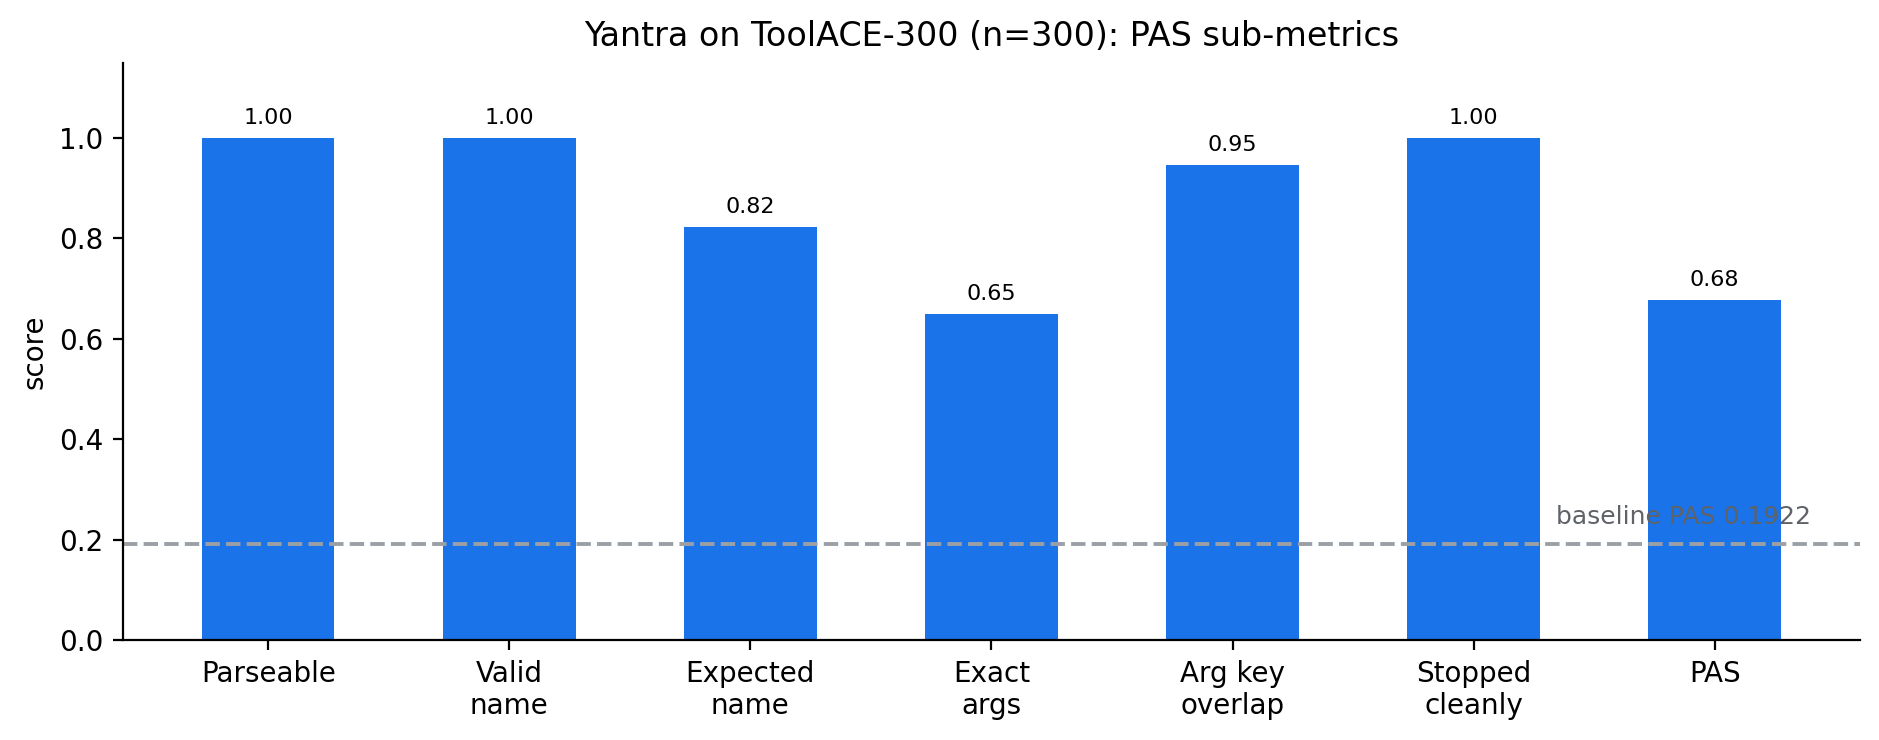
\includegraphics[width=\linewidth]{figs/pas_yantra.png}
  \caption{Yantra PAS sub-metrics on ToolACE-300. Dashed line: baseline
    PAS 0.1922 under identical serving. Baseline sub-metric bars are
    intentionally omitted (Section~\ref{sec:baseline}).}
  \label{fig:pas}
\end{figure}

Table~\ref{tab:main} and Figure~\ref{fig:pas} give the headline:
PAS \textbf{0.6775} vs.\ \textbf{0.1922} ($0.6775/0.1922 = 3.52\times$).
Every output parses; every stop is clean; argument keys are right
94.67\% of the time while exact argument values remain the headroom
at 65\% (195/300; 95\% Wilson CI 0.59--0.70). Yantra's expected-name
rate (0.8233) equals the router ceiling by construction, since the
model never selects tools.

\begin{table}[t]
  \centering
  \caption{Router benchmark on ToolACE-300 gold labels (no LLM).
    95\% Wilson intervals. The blend is the shipped default.}
  \label{tab:router}
  \begin{tabular}{lcc}
    \toprule
    Router & Accuracy & 95\% CI \\
    \midrule
    Lexical (IDF $+$ char-3-gram) & 244/300 (0.813) & 0.77--0.85 \\
    Embedding (MiniLM-L6-v2) & 242/300 (0.807) & 0.76--0.85 \\
    \textbf{Blend ($\beta{=}0.5$)} & \textbf{247/300 (0.823)}
      & \textbf{0.78--0.86} \\
    \bottomrule
  \end{tabular}
\end{table}

\begin{figure}[t]
  \centering
  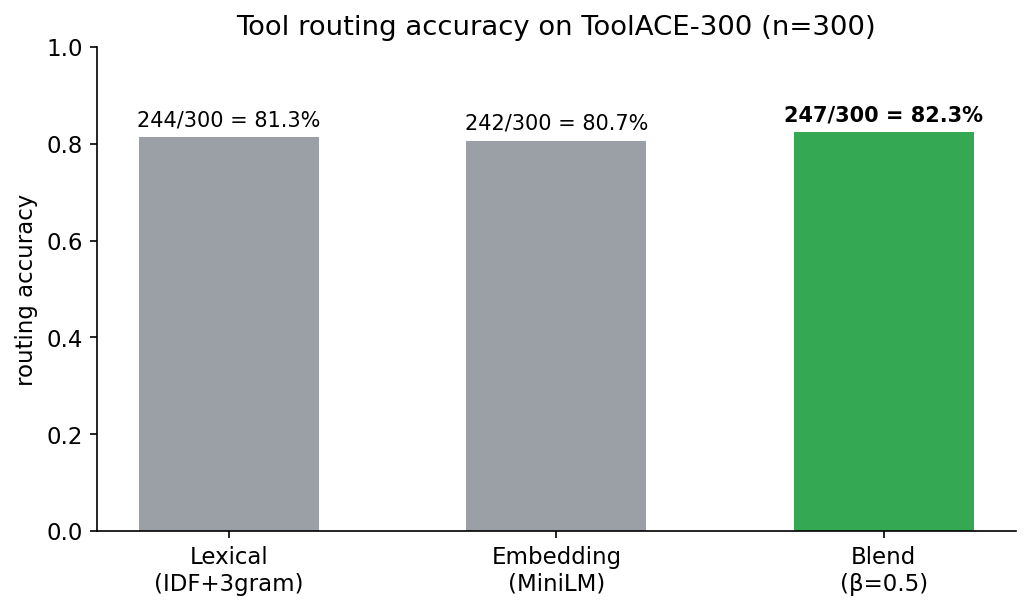
\includegraphics[width=\linewidth]{figs/router_comparison.png}
  \caption{Routing accuracy by variant. The blend recovers three
    lexical misses (244 $\to$ 247/300) with no retraining.}
  \label{fig:router}
\end{figure}

Routing (Table~\ref{tab:router}, Figure~\ref{fig:router}) confirms the
design bet: tool selection is solvable in cheap code. The intervals
overlap---we do not claim the blend is significantly better, only that
it is \emph{never worse in the benchmark} and fixes qualitatively
clear semantic misses (Section~\ref{sec:blend}), at a one-time 80\,MB
cost.

\paragraph{Upper-bound analysis.}
With perfect routing (expected\_name $= 1.0$) the PAS ceiling is
$(1 + 1 + 1 + 0.65 + 0.9467 + 1)/8 = 0.70$, since exact args
(0.65) and overlap (0.9467) are properties of the language model
alone. Yantra's 0.6775 already reaches 96.8\% of this ceiling; the
remaining gap is \emph{entirely} in argument accuracy, which is the
hard part of the problem and the target of future work at larger
scales.

%=====================================================================
\section{Analysis and Negative Results}
\label{sec:analysis}

\subsection{Where the embedding blend helps}
\label{sec:blend}

The three recovered routes are all lexical-semantic gaps, e.g.\
symptom-style queries mapping to drug-name tools and a ``VR game for
Oculus Quest'' style query mapping to a \code{getVRGame} tool whose
name shares almost no tokens with the request. Character 3-grams
cannot bridge these; MiniLM cosine can. For reference, the lexical
upgrade itself fixed 17 routes with 0 regressions in the standalone
Router V2 study (227 $\to$ 244/300); the blend adds three more
($\to$ 247/300).

\subsection{Small-data DPO collapses: a negative result}
\label{sec:negatives}

After mining 66 argument failures, we ran DPO for 3 epochs at
$5{\times}10^{-5}$ on 66 contrastive pairs. The run collapsed:
\code{exact\_args} fell 0.65 $\to$ 0.14 (PAS 0.5124) as the policy
learned to emit a single blob parameter keyed by the tool name
instead of per-key \code{<param>} elements. Sixty-six pairs are
evidently too few for contrastive updates of this size at that step
budget---the preference gradient rewards the degenerate shortcut that
is closest in KL to the reference on tiny data. We discarded all
artifacts from this round (no checkpoint ships) and report it so
others skip the configuration: \emph{do not run few-shot DPO on
structured-output models without first checking emission validity}.

\subsection{Supervised replay recovers safely}
\label{sec:replay}

Supervised fine-tuning on the same 66 fixes plus 200 replay rows
(1 epoch, $10^{-5}$) plateaued at PAS $\approx 0.6747$ with no metric
regressing: SFT-only is the safe small-data update, and replay
prevents forgetting. Fixed stop sequences independently moved stopped
cleanly 0.12 $\to$ 1.00 (PAS 0.5473 $\to$ 0.6746 pre-blend). The final
$+0.0029$ to 0.6775 comes from the embedding blend. Each gain is
small; their sum is the system.

%=====================================================================
\section{Limitations and Threats to Validity}
\label{sec:limits}

We state these plainly so the work is judged on what it is: a
1\,B-scale, single-benchmark systems recipe.
(i)~Single eval slice ($n{=}300$), single seed, greedy decoding: we
report Wilson intervals for accuracies but no multi-seed variance, and
no confidence interval for PAS itself (per-case scores for the
official run live with the run artifacts, not the repo).
(ii)~Single-call English only; recovery and multiturn PAS components
are 0 by construction---the headline 0.6775 already prices this in.
(iii)~No external-benchmark validation: BFCL and APIBank are future
work, and cross-benchmark comparisons would be invalid without a
format port. (iv)~Baseline asymmetry (Section~\ref{sec:baseline}):
the reference is strong under its native stack; our $3.52\times$ holds
under identical generic serving only. A SGLang-native rematch is the
obvious follow-up. (v)~65\% exact args means one call in three has a
wrong value: schema validation before execution is mandatory, and
high-stakes tool use (payments, medical, infrastructure) is out of
scope. (vi)~The recipe is demonstrated at 1\,B; the 7\,B scaling claim
is a hypothesis, not a result.

%=====================================================================
\section{Conclusion}
\label{sec:conclusion}

Decoupling tool selection from argument generation turns 1\,B
tool calling from a joint-reasoning problem into two tractable ones:
routing in testable code (247/300) and args-only generation in a small
fine-tune, glued by a strict stop-terminated contract. Yantra reaches
PAS 0.6775 on ToolACE-300---$3.52\times$ an identically served
reference---reproducibly on a free T4 with zero API spend. The durable
lessons are arguably the small ones: fix your stops before your
losses, blend cheap signals before training bigger ones, and never
trust few-shot contrastive updates on structured outputs. Weights,
code, and notebooks are public; the failure modes are documented next
to the wins.

%=====================================================================
\section*{Reproducibility Statement}
Pipeline, eval harness, seeds (42), decoding settings (temperature 0,
\code{max\_tokens} 768, stops in Section~\ref{sec:inference}), and
checkpoints are released at \GH{} with weights at \HF{}.
The full pipeline reruns on a free Colab T4 in about three hours;
router benchmarks rerun CPU-only in minutes. Known gaps: per-case
official scores are archived with run artifacts rather than the repo,
and the upstream ToolACE snapshot may drift (we pin our extractor and
seed; rebuild from the released slice for bit-exact comparison).

\section*{Acknowledgments}
Base model MiniCPM5-1\,B by OpenBMB; training and eval data from the
Team-ACE ToolACE release; training via Unsloth (QLoRA), inference via
llama.cpp, embeddings via sentence-transformers. We thank the authors
of these open artifacts, without which a zero-budget project of this
kind is impossible.

%=====================================================================
\begin{thebibliography}{99}

\bibitem{toolace}
Team-ACE.
\newblock ToolACE: Winning the points of LLM function calling.
\newblock \emph{arXiv preprint arXiv:2409.00920}, 2024.

\bibitem{minicpm}
Shengding Hu, Yuge Tu, Xu Han, et al.
\newblock MiniCPM: Unveiling the potential of small language models with
  scalable training strategies.
\newblock \emph{arXiv preprint arXiv:2404.06395}, 2024.

\bibitem{minicpm5}
OpenBMB.
\newblock MiniCPM5-1B model card.
\newblock \url{https://huggingface.co/openbmb/MiniCPM5-1B}, 2025.
\newblock 1.08\,B Llama-architecture causal LM, Apache-2.0, native tool
  calling via SGLang.

\bibitem{qlora}
Tim Dettmers, Artidoro Pagnoni, Ari Holtzman, and Luke Zettlemoyer.
\newblock QLoRA: Efficient finetuning of quantized LLMs.
\newblock In \emph{Advances in Neural Information Processing Systems
  (NeurIPS)}, 2023.
\newblock arXiv:2305.14314.

\bibitem{dpo}
Rafael Rafailov, Archit Sharma, Eric Mitchell, Stefano Ermon,
  Christopher~D. Manning, and Chelsea Finn.
\newblock Direct preference optimization: Your language model is secretly a
  reward model.
\newblock In \emph{Advances in Neural Information Processing Systems
  (NeurIPS)}, 2023.
\newblock arXiv:2305.18290.

\bibitem{gorilla}
Shishir~G. Patil, Tianjun Zhang, Xin Wang, and Joseph~E. Gonzalez.
\newblock Gorilla: Large language model connected with massive APIs.
\newblock \emph{arXiv preprint arXiv:2305.15334}, 2023.

\bibitem{toolllm}
Yujia Qin, Shihao Liang, Yining Ye, et al.
\newblock ToolLLM: Facilitating large language models to master 16000+
  real-world APIs.
\newblock In \emph{International Conference on Learning Representations
  (ICLR)}, 2024.
\newblock arXiv:2307.16789.

\bibitem{bfcl}
Shishir~G. Patil, Huanzhi Mao, Fanjia Yan, Charlie Cheng-Jie Ji,
  Vishnu Suresh, Ion Stoica, and Joseph~E. Gonzalez.
\newblock The Berkeley Function Calling Leaderboard (BFCL): from tool use
  to agentic evaluation of large language models.
\newblock In \emph{Proceedings of the 42nd International Conference on
  Machine Learning (ICML), PMLR 267}, 2025.

\bibitem{apibank}
Minghao Li, Feifan Song, Bowen Yu, et al.
\newblock API-Bank: A benchmark for tool-augmented LLMs.
\newblock \emph{arXiv preprint arXiv:2304.08244}, 2023.

\bibitem{react}
Shunyu Yao, Jeffrey Zhao, Dian Yu, et al.
\newblock ReAct: Synergizing reasoning and acting in language models.
\newblock In \emph{International Conference on Learning Representations
  (ICLR)}, 2023.

\bibitem{toolformer}
Timo Schick, Jane Dwivedi-Yu, Roberto Dess{\`\i}, et al.
\newblock Toolformer: Language models can teach themselves to use tools.
\newblock In \emph{Advances in Neural Information Processing Systems
  (NeurIPS)}, 2023.

\bibitem{sbert}
Nils Reimers and Iryna Gurevych.
\newblock Sentence-BERT: Sentence embeddings using Siamese BERT-networks.
\newblock In \emph{Empirical Methods in Natural Language Processing
  (EMNLP)}, 2019.

\bibitem{unsloth}
Unsloth AI.
\newblock Unsloth: Easiest tool to fine-tune LLMs.
\newblock \url{https://github.com/unslothai/unsloth}, 2024.

\bibitem{llamacpp}
Georgi Gerganov et al.
\newblock llama.cpp: LLM inference in C/C++.
\newblock \url{https://github.com/ggerganov/llama.cpp}, 2023.

\bibitem{yantra}
Gautam Kishore.
\newblock Yantra: A reproducible recipe for sub-1B agentic tool
  calling with decoupled routing.
\newblock \emph{arXiv preprint arXiv:TODO}, 2026.
\newblock Weights: \url{https://huggingface.co/eulogik/yantra-1b-agent};
  code: \url{https://github.com/eulogik/yantra}. MIT license.

\end{thebibliography}

%=====================================================================
\appendix

\section{PAS definition}
\label{app:pas}

For one case let $p \in \{0,1\}^6$ be parseable, valid name, expected
name, exact args, $\mathrm{overlap} = |K_{\mathrm{pred}} \cap
K_{\mathrm{gold}}| / |K_{\mathrm{gold}}|$ (1 if gold has no args),
stopped cleanly. With recovery and multiturn fixed at 0,
$\mathrm{PAS} = \frac{1}{8}(\sum p + 0 + 0)$.
Dataset PAS is the mean over cases. Yantra's official run:
$(1 + 1 + 0.8233 + 0.65 + 0.9467 + 1)/8 = 0.6775$.

\section{Prompt, stops, and parser}
\label{app:prompt}

The exact inference prompt (router output \code{t*} spliced in):
\begin{lstlisting}
<user>{query}</user>
<tools>[{name, description, parameters}...]</tools>
<calls><bind tool="{t*}"/>
\end{lstlisting}
Stop strings (literal newline shown as \textbackslash n):
\begin{itemize}
  \setlength{\itemsep}{0pt}
  \item \code{"\textbackslash n<bind"}, \code{"<tool\_result>"},
    \code{"<user>"}
  \item \code{"</calls>"}, \code{"<tool\_error>"},
    \code{"<reflect>"}
\end{itemize}
Parser: find all bind tags; scan binds last-to-first for the first
with a following \code{<args>} block before the next bind; parse
\code{<param>} pairs, else tagless \code{name="k">v} lines; stopped
iff trailing text after the last action-end tag is empty.

\section{Hyperparameters}
\label{app:hyper}

\begin{center}
\begin{tabular}{ll}
  \toprule
  Setting & Value \\
  \midrule
  Base & \code{openbmb/MiniCPM5-1B} (Apache-2.0) \\
  Adapter & QLoRA $r{=}64$, $\alpha{=}128$, dropout 0.05 \\
  SFT LR / epochs & $10^{-4}$, 2 (DTSA); $10^{-4}$, 1 (RTE) \\
  DPO (stage 4) & $5{\times}10^{-5}$, 1 epoch, 7,795 pairs \\
  Replay SFT & $10^{-5}$, 1 epoch, 66 fixes $+$ 200 replay \\
  Decoding & temperature 0, \code{max\_tokens} 768, $n_{\mathrm{ctx}}$ 4096 \\
  Router blend & $\beta = 0.5$, MiniLM-L6-v2 (80\,MB) \\
  Eval & ToolACE-300, seed 42, single-call English \\
  Export & Q4\_K\_M GGUF, 688\,MB \\
  \bottomrule
\end{tabular}
\end{center}

\section{Worked example}
\label{app:example}

Query: ``Find me a VR game for Oculus Quest.'' Router V2 binds
\code{getVRGame}; the model completes:
\begin{lstlisting}
<args><param name="platform">Oculus Quest</param><param name="genre">adventure</param></args><action_end/>
\end{lstlisting}
Lexical-only routing misses this case (``VR game'' shares almost no
tokens with \code{getVRGame}); the MiniLM blend recovers it---the
mechanism behind two of the three 244 $\to$ 247 routing fixes.

\end{document}
